%%=============================================================================
%% Inleiding
%%=============================================================================

\chapter{\IfLanguageName{dutch}{Inleiding}{Introduction}}%
\label{ch:inleiding}

Iedereen wordt dagelijks geconfronteerd met lezen. Deze vaardigheid strekt zich uit tot elk aspect van ons dagelijks leven, en dit geldt des te meer in het onderwijs, waar leraren worden aangemoedigd om diverse leesmaterialen te gebruiken om lesinhouden op een authentieke manier over te brengen. Wetenschappelijke artikelen kunnen ingezet worden als leesvoer voor scholieren in de derde graad van het middelbaar onderwijs, maar de leesgraad van deze artikelen brengt een nieuwe uitdaging met zich mee voor zowel scholieren als leerkrachten. 

\medspace

Het Amerikaanse onderwijs stampte C.R.E.A.T.E.\footnote{https://teachcreate.org/} uit de grond. Dit initiatief zet scholieren tussen 12 en 18 jaar aan om wetenschappelijke artikelen te lezen in plaats van enkel boeken. Daarmee komen zij in direct contact met wetenschappelijk onderzoek. Zo heeft deze doelgroep meer grip op hoe wetenschappers experimenten uitvoeren, plannen en resultaten analyseren en interpreteren. In Vlaanderen bestaat er geen gelijkaardig initiatief, maar er wordt wel vanuit de lerarenopleidingen sterk ingezet op divers didactisch leesmateriaal. Vlaamse STEM-leerkrachten in de derde graad middelbaar onderwijs moeten volgens het M-decreet en de leerplannen van zowel het katholiek\footnote{https://pro.katholiekonderwijs.vlaanderen/basisoptie-stem/ondersteunend-materiaal} als het gemeenschapsonderwijs\footnote{https://g-o.be/stem/} hun theorielessen op een toegankelijke manier aanbieden, zodat alle scholieren ongeacht leesachterstand worden meegenomen in het verhaal. 

\medspace

Vlaanderen is met een jaarlijks budget van 32 miljoen een pionier in Europa op het gebied van artificiële intelligentie (AI) op de werkvloer \autocite{Crevits2022}. Zo stampte de Vlaamse overheid verschillende AI-projecten uit de grond, om Vlaamse AI-ontwikkelingen te ondersteunen en om AI-softwarebedrijven te inspireren. Het amai!-project\footnote{https://amai.vlaanderen/} brengt AI-softwarebedrijven uit diverse domeinen, waaronder het onderwijs om processen te automatiseren en de werkdruk verminderen, zoals met real-time ondertiteling in de klas en een taalassistent voor leerkrachten in meertalige klasgroepen.


\section{\IfLanguageName{dutch}{Probleemstelling}{Problem Statement}}%
\label{sec:probleemstelling}

Iedere drie jaar wordt in ongeveer 79 geïndustrialiseerde landen de PISA-test afgenomen, die waaronder leesvaardigheid en de wetenschappelijke geletterdheid van 15-jarige scholieren, meet. Uit de enquete blijkt dat deze doelgroep zeer negatief is over leesplezier en daarmee scoort Vlaanderen het slechtst van alle bevraagde landen. Zoals aangegeven in \ref*{img:oeso-leesplezier} beschouwt bijna de helft van de bevraagden intensief lezen als tijdverspilling en slechts 17\% beschouwt lezen als een hobby. Boeiende topics kunnen belemmerd worden door deze vorm van media bij deze doelgroep.

\begin{figure}[H]
	\begin{center}
		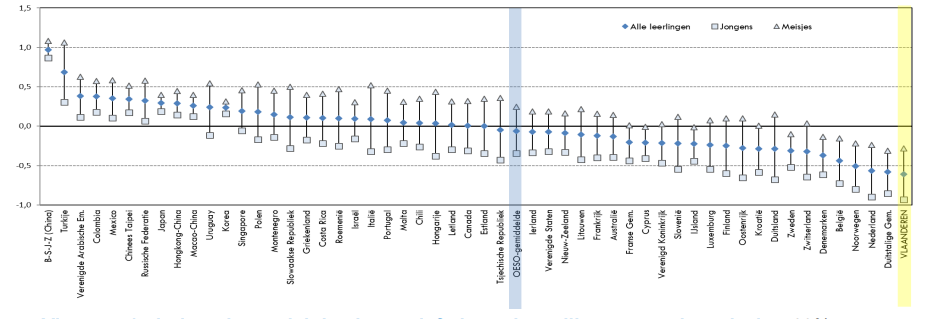
\includegraphics[width=\linewidth]{img/oeso-graphic-leesplezier.png}
	\end{center}
	\caption{Figuur van \textcite{DeMeyer2019}}
	\label{img:oeso-leesplezier}
\end{figure}

\medspace

% TODO dit toevoegen na einde van eerste zin: 
% https://www.onderwijsinspectie.be/sites/default/files/2022-06/voi_200318-Rapport_begrijpend_lezen_bao.pdf
Intensief leesbegrip valt niet te omzeilen in onze huidige samenleving, maar dit leesbegrip verschilt enorm in het middelbaar onderwijs. Een doelgroep die hier extra mee geconfronteerd wordt zijn scholieren met dyslexie. Onderzoeken van \textcite{Bonte2020, VanDerMeer2022} schatten dat ongeveer 15\% van de Vlaamse scholieren in het middelbaar onderwijs een vorm van dyslexie heeft. Zo kunnen scholieren met dyslexie bij het intensief lezen geconfronteerd worden op een moeizame en stroeve automatisering bij het lezen en spellen. Hoewel scholieren met dyslexie ondersteuning kunnen krijgen, mag de impact van leesstoornissen niet onderschat worden. De gevolgen hiervan kunnen zich namelijk doorzetten na het middelbaar onderwijs. Leesvaardigheid blijft daarmee cruciaal voor succes op school en in het werkveld. Scholieren met dyslexie kunnen hebben met spelling, wat kan leiden tot onzekerheid en stress. Daarnaast zijn vooroordelen nog steeds een probleem en kunnen ze leiden tot stigmatisering. Echter toont onderzoek aan dat scholieren met dyslexie doorzettingsvermogen hebben en goede probleemoplossers zijn \autocite{Ghesquiere2018, Lissens2020, Bonte2020}. 

\medspace

Het leerplan voor STEM-vakken stimuleert het gebruik van wetenschappelijke artikelen, maar houdt niet altijd rekening met de bijhorende complexe leesgraad. De ingewikkelde woordenschat en syntax in wetenschappelijke artikelen kunnen een hindernis vormen voor de begrijpelijkheid van een tekst, waardoor scholieren met dyslexie de kerninhoud moeilijk kunnen doorgronden. Het handmatig vereenvoudigen van wetenschappelijke artikelen echter planning, tijd en energie van leerkrachten in de derde graad middelbaar onderwijs opslorpen. Het Vlaamse middelbaar onderwijs staat onder druk en docenten hebben moeite om met deze werkdruk boven water te blijven. 

\medspace

Nu is AI technologisch hoogstaand om tekstvereenvoudiging te automatiseren en om een baanbrekende oplossing aan te bieden aan het middelbaar onderwijs. Enerzijds om de werkdruk bij leerkrachten te verminderen, anderzijds om scholieren in de derde graad te ondersteunen bij het lezen van complexe wetenschappelijke artikelen. Voor het gebruik van taalmodellen of API's is uitgebreide informaticakennis nodig, die de meeste scholieren en leraren niet hebben. Anderzijds zijn tools te beperkt en eerder gericht op samenvatten wat niet noodzakelijk bijdraagt tot een eenvoudigere tekst. Er is nood aan een intuïtieve en gebruikersvriendelijke toepassing die taalmodellen of API's kan integreren en aanpassen naargelang de specifieke behoeften van een student met dyslexie.

\section{\IfLanguageName{dutch}{Onderzoeksvraag}{Research question}}%
\label{sec:onderzoeksvraag}

De volgende onderzoeksvraag is opgesteld: Hoe kan een wetenschappelijke artikel automatisch vereenvoudigd worden, gericht op de unieke noden van scholieren met dyslexie in de derde graad middelbaar onderwijs?. Om deze onderzoeksvraag te kunnen beantwoorden, moet een antwoord gezocht worden op de volgende deelvragen:

\begin{enumerate}
	% 1
	\item Welke specifieke noden hebben scholieren met dyslexie van de derde graad middelbaar onderwijs bij het begrijpen van complexere teksten? Aanvullend hierop: 
	\begin{itemize}
		\item Wat zijn de specifieke kenmerken van wetenschappelijke artikelen?
	\end{itemize} 
	% 2
	\item Welke aanpakken zijn er voor geautomatiseerde tekstvereenvoudiging?
	\begin{itemize}
		\item Hoe worden teksten handmatig vereenvoudigd voor scholieren met dyslexie?
		\item Welke toepassingen, tools en modellen zijn er beschikbaar om Nederlandse geautomatiseerde tekstvereenvoudiging met AI mogelijk te maken?
		\item Hoe kunnen geautomatiseerde tekstvereenvoudiging en gepersonaliseerde tekstvereenvoudiging gecombineerd worden?
	\end{itemize}
	%3 
	\item Met welke valkuilen bij taalverwerking met AI moeten ontwikkelaars rekening houden?
	%4 
	\item Welke functies ontbreken AI-toepassingen om geautomatiseerde tekstvereenvoudiging mogelijk te maken voor scholieren met dyslexie in de derde graad middelbaar onderwijs? 
	\begin{itemize}
		\item Welke manuele methoden voor tekstverereenvoudiging komen niet in deze tools voor?"
	\end{itemize}
	% 5
	\item Welke taalmodellen of LLM's zijn geschikt voor automatische tekstvereenvoudiging voor vereenvoudigde wetenschappelijke artikelen voor scholieren met dyslexie in de derde graad van het middelbaar onderwijs met dezelfde of gelijkaardige kwaliteiten als manuele tekstvereenvoudiging?
	% 6
	\item Hoe kan een intuïtieve lokale webtoepassing worden ontwikkeld die zowel scholieren met dyslexie als docenten helpt bij het vereenvoudigen van wetenschappelijke artikelen met behoud van semantiek, jargon en zinsstructuren?
\end{enumerate}


\section{\IfLanguageName{dutch}{Onderzoeksdoelstelling}{Research objective}}%
\label{sec:onderzoeksdoelstelling}

Het onderzoek heeft als doel om de technologische en logopedische aspecten te identificeren die AI-ontwikkelaars in overweging moeten nemen bij het creëren van een op maat gemaakte AI-toepassing voor geautomatiseerde tekstvereenvoudiging, specifiek ontwikkeld voor scholieren in de derde graad. Het resultaat van dit onderzoek is een prototype voor een AI-toepassing voor tekstvereenvoudiging in de vorm van een webtool. De webtool heeft twee functies. Enerzijds kan de tool de inhoud van wetenschappelijke artikelen vereenvoudigen op basis van de specifieke behoeften van scholieren met dyslexie in de derde graad van het middelbaar onderwijs. Anderzijds biedt de tool een geautomatiseerde benadering voor lectoren om wetenschappelijke artikelen te vereenvoudigen op basis van geselecteerde parameters en deze vervolgens in een bruikbaar formaat (pdf of word) terug te geven. De invoer bij dit prototype is een wetenschappelijk artikel in tekst- of PDF-formaat.


\section{\IfLanguageName{dutch}{Opzet van deze bachelorproef}{Structure of this bachelor thesis}}%
\label{sec:opzet-bachelorproef}

De rest van deze bachelorproef is als volgt opgebouwd:

In Hoofdstuk~\ref{ch:stand-van-zaken} wordt een overzicht gegeven van de stand van zaken binnen het onderzoeksdomein, op basis van een literatuurstudie.

In Hoofdstuk~\ref{ch:methodologie} wordt de methodologie toegelicht en worden de gebruikte onderzoekstechnieken besproken om een antwoord te kunnen formuleren op de onderzoeksvragen. Eerst wordt er een requirementsanalyse uitgevoerd, gevolgd door de ontwikkeling van een prototype voor tekstvereenvoudiging.

\begin{enumerate}
	% 1
	\item Welke specifieke noden hebben scholieren met dyslexie van de derde graad middelbaar onderwijs bij het begrijpen van complexere teksten? Aanvullend hierop: 
	\begin{itemize}
		\item Wat zijn de specifieke kenmerken van wetenschappelijke artikelen?
	\end{itemize} 
	% 2
	\item Welke aanpakken zijn er voor geautomatiseerde tekstvereenvoudiging?
	\begin{itemize}
		\item Hoe worden teksten handmatig vereenvoudigd voor scholieren met dyslexie?
		\item Welke toepassingen, tools en modellen zijn er beschikbaar om Nederlandse geautomatiseerde tekstvereenvoudiging met AI mogelijk te maken?
		\item Hoe kunnen geautomatiseerde tekstvereenvoudiging en gepersonaliseerde tekstvereenvoudiging gecombineerd worden?
	\end{itemize}
	%3 
	\item Met welke valkuilen bij taalverwerking met AI moeten ontwikkelaars rekening houden?
	%4 
	\item Welke functies ontbreken AI-toepassingen om geautomatiseerde tekstvereenvoudiging mogelijk te maken voor scholieren met dyslexie in de derde graad middelbaar onderwijs? 
	\begin{itemize}
		\item Welke manuele methoden voor tekstverereenvoudiging komen niet in deze tools voor?"
	\end{itemize}
	% 5
	\item Welke taalmodellen of LLM's zijn geschikt voor automatische tekstvereenvoudiging voor vereenvoudigde wetenschappelijke artikelen voor scholieren met dyslexie in de derde graad van het middelbaar onderwijs met dezelfde of gelijkaardige kwaliteiten als manuele tekstvereenvoudiging?
	% 6
	\item Hoe kan een intuïtieve lokale webtoepassing worden ontwikkeld die zowel scholieren met dyslexie als docenten helpt bij het vereenvoudigen van wetenschappelijke artikelen met behoud van semantiek, jargon en zinsstructuren?
\end{enumerate}

In Hoofdstuk~\ref{ch:discussie} worden de resultaten gegeven op dit onderzoek. In Hoofdstuk~\ref{ch:conclusie}, tenslotte, wordt de conclusie gegeven en een antwoord geformuleerd op de onderzoeksvragen. Daarbij wordt ook een aanzet gegeven voor toekomstig onderzoek binnen dit domein.